\begin{frame}[allowframebreaks]{VideoAdapter}
DDPMs as Energy-Based Models (EBMs)
\begin{figure}
    \centering
    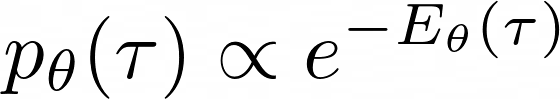
\includegraphics[width=0.35\linewidth,height=\textheight,keepaspectratio]{images/adv-img-gen/slide_162_1_img.png}
\end{figure}
\vspace{1em}
Since the denoising function ($\epsilon$) models the score, we have
\begin{figure}
    \centering
    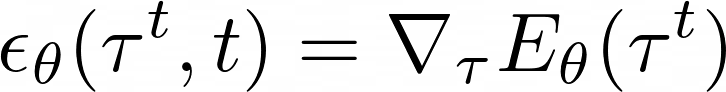
\includegraphics[width=0.4\linewidth,height=\textheight,keepaspectratio]{images/adv-img-gen/slide_162_2_img.png}
\end{figure}

\framebreak
Learn a distribution as a product of a pretrained (large) model and domain specific (small) model
\begin{figure}
    \centering
    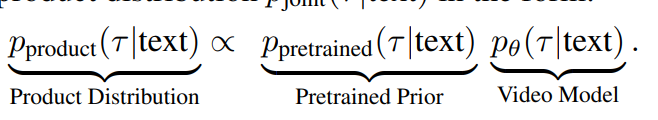
\includegraphics[width=0.7\linewidth,height=\textheight,keepaspectratio]{images/adv-img-gen/slide_163_1_img.png}
\end{figure}
\begin{figure}
    \centering
    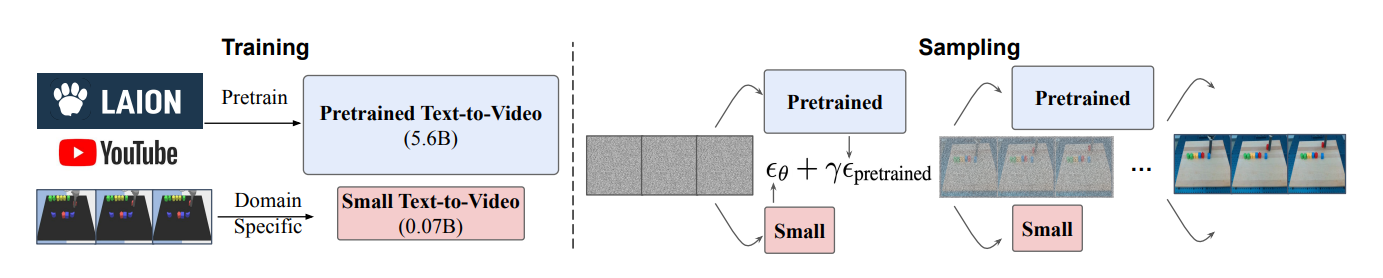
\includegraphics[width=1.05\linewidth,height=\textheight,keepaspectratio]{images/adv-img-gen/slide_163_2_img.png}
\end{figure}

\framebreak
Under the product assumption, we can use the EBM interpretation to combine the scores of the diffusion models
\vspace{1em}
\begin{figure}
    \centering
    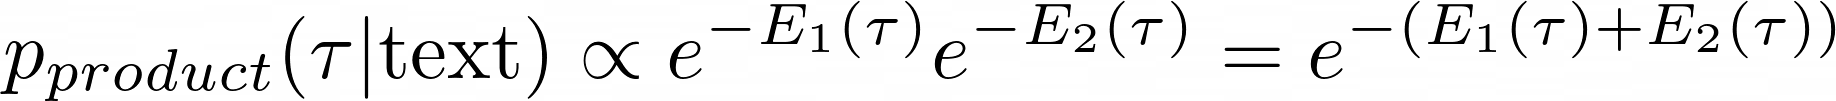
\includegraphics[width=\linewidth,height=\textheight,keepaspectratio]{images/adv-img-gen/slide_164_1_img.png}
\end{figure}
\vspace{1em}
\begin{figure}
    \centering
    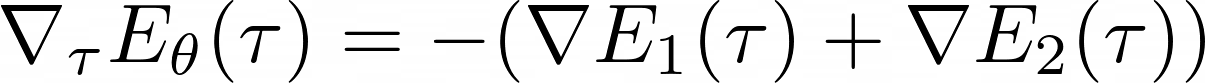
\includegraphics[width=0.7\linewidth,height=\textheight,keepaspectratio]{images/adv-img-gen/slide_164_2_img.png}
\end{figure}

\framebreak
\begin{figure}
    \centering
    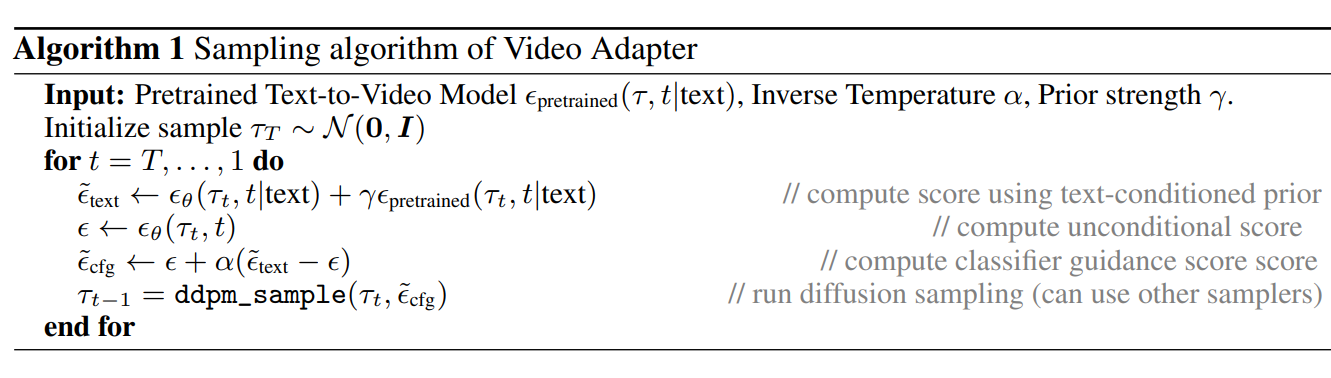
\includegraphics[width=\linewidth,height=\textheight,keepaspectratio]{images/adv-img-gen/slide_165_1_img.png}
\end{figure}

\framebreak
\begin{figure}
    \centering
    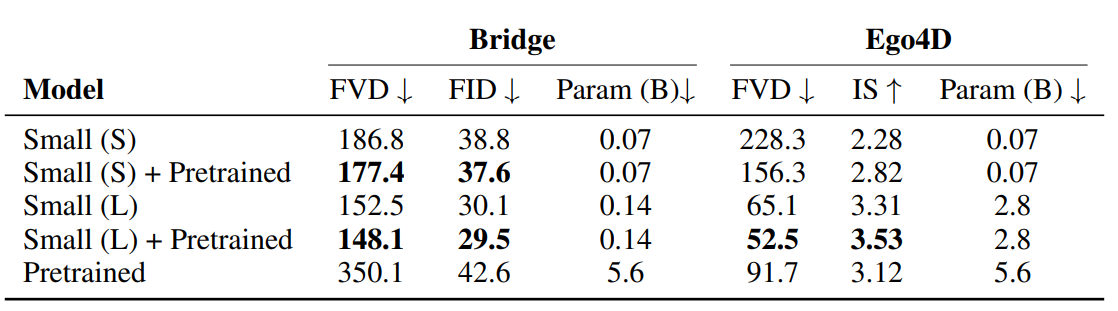
\includegraphics[width=\linewidth,height=\textheight,keepaspectratio]{images/adv-img-gen/slide_166_1_img.png}
\end{figure}

\framebreak
Can adapt to different domains (robot trajectories, ego-centric camera)
\begin{columns}
    \column{0.5\textwidth}
    \begin{figure}
        \centering
        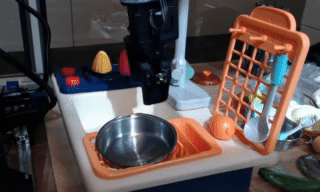
\includegraphics[width=\linewidth,height=\textheight,keepaspectratio]{images/adv-img-gen/slide_167_1_img.png}
        \caption*{\href{https://drive.google.com/file/d/1l3UCX-6TzMOqymeQwu3aYdPopSxV64cr/view?usp=sharing}{Link: GIFF}}
    \end{figure}
    \column{0.5\textwidth}
    \begin{figure}
        \centering
        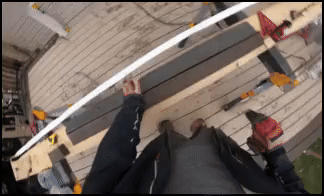
\includegraphics[width=\linewidth,height=\textheight,keepaspectratio]{images/adv-img-gen/slide_167_2_img.png}
        \caption*{\href{https://drive.google.com/file/d/15EoGTelZTxyMg6kLnoQc2PmlkRn1OTB8/view?usp=sharing}{Link: GIFF}}
    \end{figure}
\end{columns}
\end{frame}